\chapter{\uppercase{GENERATION OF THE ANOMALY DETECTION MECHANISM}}
\label{Capitulo 5}

This chapter describes the process that was followed to generate the conduction anomaly detection mechanism. As reviewed in Chapter 3, in this document, an outlier detector with a semi-supervised approach is proposed; however, before delving into the proposed method, a description of the development environment with which the experiment was used should be carried out, in addition to reviewing dataset available in this study.
%Este cap\'{i}tulo describe el proceso que se sigui\'{o} para la generaci\'{o}n del mecanismo de detecci\'{o}n de anomal\'{i}as de conducci\'{o}n. Seg\'{u}n lo repasado en el cap\'{i}tulo 3, en el presente trabajo, se propone un detector de valores at\'{i}picos con un enfoque semi-supervisado; sin embargo, antes de profundizar en el m\'{e}todo propuesto se debe realizar una descripci\'{o}n del entorno de desarrollo con el se que desarroll\'{o} el experimento, adem\'{a}s de realizar un repaso del conjunto de datos con el que se cuenta en este estudio.

\section{Development environment}

The experiment of this study was developed on a laptop with following characteristics:
%El experimento de este estudio fue desarrollado en una computador port\'{a}til con las siguientes caracter\'{i}sticas:

\begin{itemize}
\item Intel Core i5-5200U 2.2GHz processor (c / TB 2.7 GHz).
\item 8 GB of RAM.
\item ArchLinux Operating System version 4.15.15-1-ARCH (64 bits).
%\item Procesador Intel Core i5-5200U 2.2GHz (c/TB 2.7 GHz).
%\item 8 GB de memoria RAM.
%\item Sistema Operativo ArchLinux version 4.15.15-1-ARCH (64 bits). 
\end{itemize}

It is important to clarify that methods' types used in this study are usually much more efficient in computers that have a graphics processing unit (GPU), since this unit allows parallel processing. The code developed in this work was written in \textsc{PYTHON}, an interpreted programming language that emphasizes code simplicity and readability, as well as being powered with support of powerful scientific libraries such as \textsc{NUMPY}, \textsc{SCIPY}, \textsc{OPENCV}, \textsc{KERAS}, \textsc{MATPLOTLIB}, \textsc{SEABORN}, etc. as for the experiments' development and the generation of detection mechanism, Jupyter Notebook was used, which is a local Python-based web application that allows you to view and execute documents that contain source code and equations. The versions of tools used are detailed below.
%Es importante aclarar que el tipo de m\'{e}todos utilizado en este estudio suelen ser mucho m\'{a}s eficientes en computadores que cuenten con una unidad de procesamiento gr\'{a}fico (GPU), dado que esta unidad permite el procesamiento en paralelo. El c\'{o}digo desarrollado en este trabajo fue escrito en \textsc{Python}, un lenguaje de programaci\'{o}n interpretado que se enfatiza en la simplicidad y legibilidad de c\'{o}digo, adem\'{a}s de que se potencia con el apoyo de poderosas librer\'{i}as cient\'{i}ficas tales como \textsc{NumPy}, \textsc{SciPy}, \textsc{OpenCV}, \textsc{Keras}, \textsc{Matplotlib}, \textsc{Seaborn}, etc. En cuanto al desarrollo de experimentos y la generaci\'{o}n del mecanismo de detecci\'{o}n esta desarrollado en Jupyter Notebook que es una aplicaci\'{o}n web local basado en Python que permite visualizar y ejecutar documentos que contienen c\'{o}digo fuente y ecuaciones. Las versiones de las herramientas utilizadas son detalladas a continuaci\'{o}n:

\begin{itemize}
\item \textbf{Python:} 3.6.5

\item \textbf{Jupyter:} 4.3

\item \textbf{Keras:} 2.2.2

\item \textbf{Tensorflow:} 1.11.0

\item \textbf{Scikit-learn:} 0.19.1

\item \textbf{Matplotlib:} 2.0.2
\end{itemize}

\section{Normal and anomalous dataset}

In Chapter 4 capturing's process and preparing dataset was described, as well as its division into training/development/test set; however, it should be noted that in that chapter was focused only on the normal dataset.
%En el Cap\'{i}tulo 4 se describi\'{o} el proceso de captura y preparaci\'{o}n del conjunto de datos, as\'{i} como tambi\'{e}n su divisi\'{o}n en conjunto de entrenamiento/desarrollo/prueba; sin embargo cabe aclarar que aquel cap\'{i}tulo s\'{o}lo se enfoc\'{o} en el \textbf{conjunto de datos normales}.%, con los cuales se entrenar\'{a} el modelo ajustado al comportamiento normal.%; por lo que es el conjunto que se usa para entrenar el modelo que se ajusta al comportamiento normal de manejo.

\vspace{5mm} %5mm vertical space

Although there is a large amount of normal data, it is necessary to collect samples corresponding to anomalies, in order to validate the method proposed in this project. Therefore, the capture of a anomalous dataset was carried out, which is compose according to Table \ref{table:conjunto_anomalias}.
%A pesar de que se cuenta con una gran cantidad de datos normales, es necesario recolectar muestras que corresponden a anomal\'{i}as, con el objetivo de poder validar el m\'{e}todo que se propone en este proyecto. Por lo tanto, se realiz\'{o} la captura de un conjunto de \textbf{datos an\'{o}malos}, el cual est\'{a} conformado seg\'{u}n el Cuadro \ref{table:conjunto_anomalias}.

\begin{table}[H]
\centering
\begin{tabular}{|l|l|l|}
\hline
\textbf{Anomaly's type} & \textbf{No. anomalies} & \textbf{No. data} \\ \hline
Zig Zag turns & 5 & 105  \\ \hline
Right and left turns at high speed & 7 & 35  \\ \hline
Dry brakes & 6 & 24 \\ \hline
\end{tabular}
\caption{Table of anomaly dataset (Own elaboration).}
\label{table:conjunto_anomalias}
\end{table}

\vspace{5mm} %5mm vertical space

As mentioned in previous paragraph, anomaly set was captured to validate the proposed method, therefore this set was labeled as positive (with label 1) and normal dataset as negative (with label 0).
%Como se mencion\'{o} en el p\'{a}rrafo anterior el conjunto de anomal\'{i}as fue capturado para validar el m\'{e}todo propuesto, por lo tanto este conjunto se etiquet\'{o} como positivo (con la etiqueta 1) y el conjunto de datos normales como negativo (con la etiqueta 0).

\subsection{Generation of time series}

For the generation of anomaly detector model, it was decided to go beyond a simple point anomalies' detection and thus be able to detect contextual or collective anomalies; due to this, the use of data in time series is required.
%Para la generaci\'{o}n del modelo detector de anomal\'{i}as se decidi\'{o} ir m\'{a}s all\'{a} de una simple detecci\'{o}n de anomal\'{i}as puntuales y as\'{i} poder detectar anomal\'{i}as contextuales o colectivas; debido a ello se requiere el uso de datos en series de tiempo.

\vspace{5mm} %5mm vertical space

Data captured by mobile device is dependent on chronometric time in which it was captured (one data per second); therefore, first step is generate small time series fractions. In Figure \ref{fig:series-de-tiempo} results of different time series' sizes are presented, observing these results in first instance, the time series that has two steps are discarded; because they are not descriptive enough. As for remaining time series, it is not possible to define yet what is the correct number of steps, therefore, it will be a parameter to optimize in the different experiments that will be carried out in following sections. It should be noted that domain of this variable is between 3 and 5 steps.
%Los datos capturados por el dispositivo m\'{o}vil, son dependientes del tiempo cronom\'{e}trico en el que fueron capturados (un dato por segundo); por lo cual el primer paso a realizar es la generaci\'{o}n de peque\~{n}as fracciones de series temporales. En la Figura \ref{fig:series-de-tiempo} se presenta los resultados de diferentes tama\~{n}os de series de tiempo, observando estos resultados en primera instancia se descarta la serie de tiempo que cuenta con dos pasos; debido a que no es lo suficientemente descriptiva. En cuanto a las series de tiempo restantes no es posible definir a\'{u}n cual es la cantidad correcta de pasos, por lo cual, ser\'{a} un par\'{a}metro a optimizar en los diferentes experimentos que se realizar\'{a} en las siguientes secciones. Cabe recalcar que el dominio de \'{e}sta variable est\'{a} entre 3 y 5 pasos.

\begin{figure}[H]
        \centering
\fbox{\begin{varwidth}{\textwidth}
        \centering
        \begin{subfigure}[h]{0.45\textwidth} 
            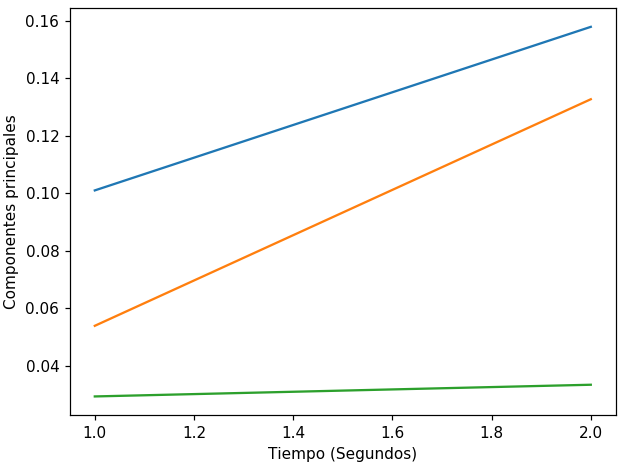
\includegraphics[width=\textwidth]{imagenes/Cap4/pca3-2}
            \caption{2\-step time series.}
            \label{fig:pasos2}
        \end{subfigure}       
        \begin{subfigure}[h]{0.45\textwidth} 
            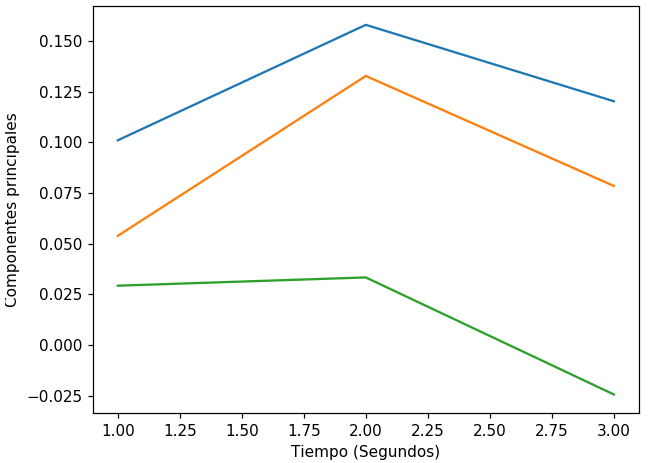
\includegraphics[width=\textwidth]{imagenes/Cap4/pca3-3}
            \caption{3\-step time series.}
            \label{fig:pasos3}
        \end{subfigure}
        \begin{subfigure}[h]{0.45\textwidth} 
            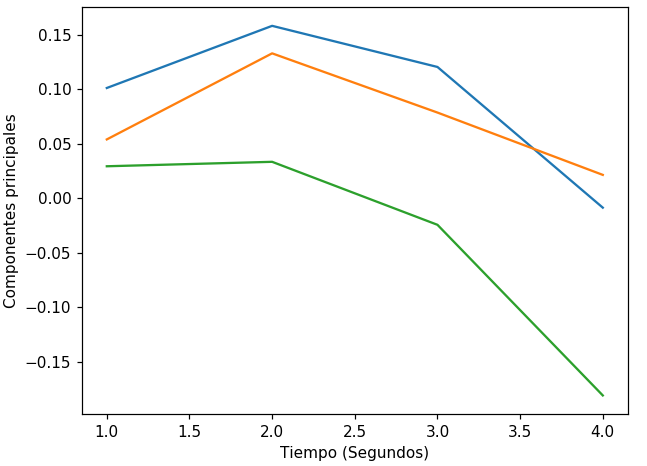
\includegraphics[width=\textwidth]{imagenes/Cap4/pca3-4}
            \caption{4\-step time series.}
            \label{fig:pasos4}
        \end{subfigure}       
        \begin{subfigure}[h]{0.45\textwidth} 
            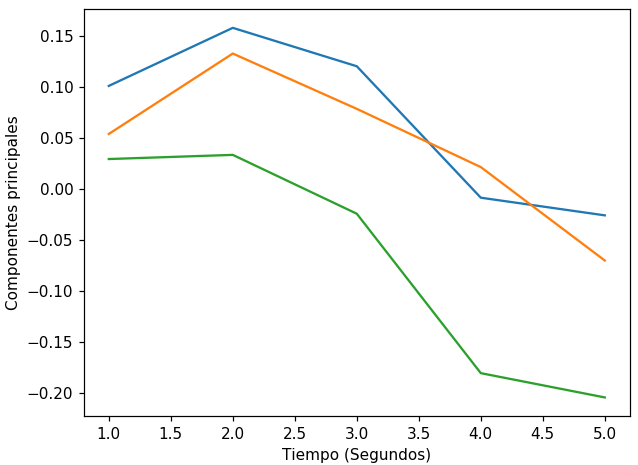
\includegraphics[width=\textwidth]{imagenes/Cap4/pca3-5}
            \caption{5\-step time series.}
            \label{fig:pasos5}
        \end{subfigure}
        \end{varwidth}}
        \caption{Results from different sizes of time series (Own elaboration).}
		\label{fig:series-de-tiempo}
    \end{figure}
    
\section{Anomaly detection model}

Present investigation proposes a method of detecting conduction anomalies following a semi-supervised approach, which consists of two components: a \textbf{normal behavior's model} and a \textbf{method for outliers' detection}.
%La presente investigaci\'{o}n propone un m\'{e}todo de detecci\'{o}n de anomal\'{i}as de conducci\'{o}n siguiendo un enfoque semi-supervisado, el cual consta de dos componentes: un \textbf{modelo del comportamiento normal} y un \textbf{m\'{e}todo para la detecci\'{o}n de valores at\'{i}picos}.

\vspace{5mm} %5mm vertical space

Therefore, a comparison was made between 3 different detection methods, and according to each's performance, the best option was chosen. Table \ref{table:metodos_comparados} presents the three different methods that were compared; where it can be seen that in all cases an autoencoder is used as a normal behavior's model, in this way, following sections will describe the choice of autoencoder and the choice of one of three different proposed anomaly detection methods.
%Por lo tanto, se realiz\'{o} la comparaci\'{o}n entre 3 diferentes m\'{e}todos de detecci\'{o}n, y seg\'{u}n el rendimiento de cada uno se elegi\'{o} la mejor opci\'{o}n. En el Cuadro \ref{table:metodos_comparados} se presenta los tres diferentes m\'{e}todos que fueron comparados; donde se puede observar que en todos los casos se usa un autoencoder como modelo del comportamiento normal, de esta manera, las siguientes secci\'{o}nes describir\'{a}n la elecci\'{o}n del autoencoder y la elecci\'{o}n de uno de los tres diferentes m\'{e}todos de detecci\'{o}n de anomal\'{i}as propuestos.

\begin{table}[H]
\centering
\begin{tabular}{|l|p{100mm}|}
\hline
\textbf{Method} & \textbf{Description} \\ \hline
AE\_T & Detection method based on autoencoders and thresholding. \\ \hline
AE\_IF & Detection method based on autoencoders and application of Isolation Forest. \\ \hline
AE\_OC-SVM & Detection method based on autoencoders and application of One-Class SVM. \\ \hline
\end{tabular}
\caption{Table of compared methods (Own elaboration).}
\label{table:metodos_comparados}
\end{table}

\subsection{Normal behavior model}

This stage is one of the most important parts of this work, because performance of anomaly detection model depends largely on precision of this stage.
%Esta etapa es una de las partes m\'{a}s importantes de \'{e}ste trabajo, debido a que el rendimiendo del modelo de detecci\'{o}n de anomal\'{i}as depende en gran parte de la precisi\'{o}n de esta etapa.

\subsubsection{Model architecture}

As mentioned in previous section, at this stage an autoencoder will be used as a model adjusted to normal driving behavior. So the autoencoder was trained with normal dataset, so that model learns to generate only the classes that are considered normal and, hopefully, it will have problems to reconstruct anomalies, because these samples were not presented during training.
%Como se mencion\'{o} en la anterior secci\'{o}n en esta etapa se utilizar\'{a} un autoencoder como modelo ajustado al comportamiento normal de conducci\'{o}n. Por lo cual el autoencoder se entren\'{o} con el conjunto de datos normales, de manera que el modelo aprenda a generar s\'{o}lo las clases que se consideran normales y, con suerte, tendr\'{a} problemas para reconstruir anomal\'{i}as, debido a que estas muestras no fueron presentadas durante el entrenamiento.

\vspace{5mm} %5mm vertical space

To do this, different architectures were tested, first the simplest way that is based only in the use of dense (fully connected) layers, then tests were carried out with convolutional networks and finally with recurrent networks making specific use of LSTM layers. For each network's type, tests was performed with 3 different types of input, that is, a different number of steps (between 3 and 5) were tested in the time series. Therefore, 9 different experiments were carried out, of which for each network's type one stood out (using networks' precision as a type of evaluation to develop comparisons).
%Para ello se prob\'{o} con diferentes arquitecturas, primero la forma m\'{a}s simple que s\'{o}lo se basa el uso de capas densas (completamente conectadas), luego se hizo pruebas con redes convolucionales y por \'{u}ltimo con redes recurrentes haciendo uso espec\'{i}fico de capas LSTM. Por cada tipo de red se hizo la prueba con 3 diferentes tipos de entrada, es decir, se prob\'{o} una diferente cantidad de pasos (entre 3 y  5) en las series temporales. Por lo tanto se realizaron 9 diferentes experimentos, de los cuales por cada tipo de red sobresali\'{o} una (usando la precisi\'{o}n de las redes como tipo de evaluaci\'{o}n para desarrollar las comparaciones).

\vspace{5mm} %5mm vertical space

Table \ref{table:dense33} shows the network that obtained the best result of all Dense Networks that were tested, this network corresponds to network that was fed with 3\-step sequences. This network has an input layer, an Flattening layer (Flatten) this because input layer receives a two-dimensional input, a set of dense layers (Dense) that compress information of input data to later rebuild them, and finally output layer is only a layer to modify the shape of output (Reshape); another important point to highlight is that inner layers use $elu$ as activation function and last dense layer uses a tangential activation function ($tanh$), this is because data set, after obtaining principal components, is found in range $(1, -1)$.
%En el Cuadro \ref{table:dense33} se presenta la red que obtuvo el mejor resultado de todas las Redes Densas que se probaron, esta red corresponde a la red que fue alimentada con secuencias de 3 pasos. Esta red cuenta con una capa de entrada (Input), una capa de aplanamiento (Flatten) esto debido a que la capa de entrada recibe una entrada bidimensional, un conjunto de capas densas (Dense) que van comprimiendo la informaci\'{o}n de los datos de entrada para posteriormente reconstruirlos, y por \'{u}ltimo la capa de salida es solo una capa para modificar la forma de la salida (Reshape); otro punto importante a resaltar es que las capas internas usan $elu$ como funci\'{o}n de activaci\'{o}n y la \'{u}ltima capa densa utilizan una funci\'{o}n de activaci\'{o}n tangencial ($tanh$), esto se debe a que el conjunto de datos, posterior a la obtenci\'{o}n de componentes principales, se encuentra en el rango $(1, -1)$.

\begin{table}[H]
\centering
\begin{center}
\begin{tabular}{ll|l|r|l|r|}
\cline{3-6}
                                                    &                             & \multicolumn{4}{c|}{\textbf{Dense Architecture}}                                                                                                           \\ \cline{3-6} 
                                                    &                             & \multicolumn{4}{c|}{\textbf{NN\_33}}                                                                                                                                   \\ \cline{3-6} 
                                                    &                             & \multicolumn{1}{c|}{\textbf{Type}} & \multicolumn{1}{c|}{\textbf{Output}} & \multicolumn{1}{c|}{\textbf{Activation}} & \multicolumn{1}{l|}{\textbf{\# Parameters}} \\ \hline
\multicolumn{1}{|l|}{\multirow{7}{*}{\textbf{PCA}}} & \multirow{7}{*}{\textbf{3}} & Input                              & (3,3)                                &                                          & 0                                           \\ \cline{3-6} 
\multicolumn{1}{|l|}{}                              &                             & Flatten                            & 9                                    &                                          & 0                                           \\ \cline{3-6} 
\multicolumn{1}{|l|}{}                              &                             & Dense                              & 8                                   & elu                                     & 80                                          \\ \cline{3-6} 
\multicolumn{1}{|l|}{}                              &                             & Dense                              & 5                                   & elu                                     & 45                                          \\ \cline{3-6} 
\multicolumn{1}{|l|}{}                              &                             & Dense                              & 8                                    & elu                                     & 88                                          \\ \cline{3-6} 
\multicolumn{1}{|l|}{}                              &                             & Dense                              & 9                                    & tanh                                     & 81                                          \\ \cline{3-6} 
\multicolumn{1}{|l|}{}                              &                             & Reshape                            & (3,3)                                &                                          & 0                                           \\ \hline
\end{tabular}
\end{center}
\caption{Dense architecture for a 3\-steps sequence and 3 principal components (Own elaboration).}
\label{table:dense33}
\end{table}

% ejemplos de cuadros de aruqitecturas de redes https://webthesis.biblio.polito.it/10360/1/tesi.pdf

% metricas de evaluacion http://www.diva-portal.org/smash/get/diva2:1225367/FULLTEXT01.pdf  , https://escholarship.org/content/qt1f03f6hb/qt1f03f6hb.pdf  ,   http://www.nada.kth.se/~ann/exjobb/maxim_wolpher.pdf

% Ejemplo cuadros resultados    https://arxiv.org/pdf/1809.00957.pdf 

On the other hand, table \ref{table:cnn33} presents network that obtains the best precision of all Convolutional Networks that were tested, this network, like previous one, corresponds to network that was fed with 3\-step sequences. Its architecture consists of an input layer (Input), a combination of one-dimensional convolution layers (Conv1D) and grouping (MaxPooling1D) until data is compressed to a dimension of (2,4), then a set of convolutional layers and upstream sample (Upsampling1D) to decode compressed information. It should be noted that this network also uses tangential activation function in its last layer for reasons explained in previous paragraph.
%Por otra parte el Cuadro \ref{table:cnn33} se presenta la red que obtiene la mejor precisi\'{o}n de todas las Redes Convolucionales que fueron probadas, esta red al igual que la anterior corresponde a la red que fue alimentada con secuencias de 3 pasos. Su arquitectura consta de una capa de entrada (Input), una combinaci\'{o}n de capas de convoluci\'{o}n de una dimensi\'{o}n (Conv1D) y agrupaci\'{o}n (MaxPooling1D) hasta comprimir los datos a una dimensi\'{o}n de (2,4), luego un conjunto de capas convolucionales y de muestra ascendente (Upsampling1D) para decodificar la informaci\'{o}n compresa. Cabe recalcar que esta red tambi\'{e}n usa la funci\'{o}n de activaci\'{o}n tangencial en su \'{u}ltima capa por las razones que se explicaron en el p\'{a}rrafo anterior.

\begin{table}[H]
\centering
\begin{center}
\begin{tabular}{ll|l|r|l|r|}
\cline{3-6}
                                                    &                             & \multicolumn{4}{c|}{\textbf{Convolutional Architecture}}                                                                                                           \\ \cline{3-6} 
                                                    &                             & \multicolumn{4}{c|}{\textbf{CNN\_33}}                                                                                                                                  \\ \cline{3-6} 
                                                    &                             & \multicolumn{1}{c|}{\textbf{Type}} & \multicolumn{1}{c|}{\textbf{Output}} & \multicolumn{1}{c|}{\textbf{Activation}} & \multicolumn{1}{l|}{\textbf{\# Parameters}} \\ \hline
\multicolumn{1}{|l|}{\multirow{8}{*}{\textbf{PCA}}} & \multirow{8}{*}{\textbf{3}} & Input                              & (3,3)                                &                                          & 0                                           \\ \cline{3-6} 
\multicolumn{1}{|l|}{}                              &                             & Conv1D                             & (3,2)                                & elu                                     & 20                                          \\ \cline{3-6} 
\multicolumn{1}{|l|}{}                              &                             & MaxPooling1D                       & (2,2)                                &                                          & 0                                           \\ \cline{3-6} 
\multicolumn{1}{|l|}{}                              &                             & Conv1D                             & (2,4)                                & elu                                     & 28                                          \\ \cline{3-6} 
\multicolumn{1}{|l|}{}                              &                             & MaxPooling1D                       & (1,4)                                &                                          & 0                                           \\ \cline{3-6} 
\multicolumn{1}{|l|}{}                              &                             & Conv1D                             & (1,6)                                & elu                                     & 54                                          \\ \cline{3-6} 
\multicolumn{1}{|l|}{}                              &                             & UpSampling1D                       & (3,6)                                &                                          & 0                                           \\ \cline{3-6} 
\multicolumn{1}{|l|}{}                              &                             & Conv1D                             & \multicolumn{1}{l|}{(3,3)}           & tanh                                     & 57                                          \\ \hline
\end{tabular}
\end{center}
\caption{Convolutional architecture for a 3\-steps sequence and 3 principal components (Own elaboration).}
\label{table:cnn33}
\end{table}

Table \ref{table:rnn33} shows network that obtained the best precision of all Recurring Networks tested, as previous cases, this network is fed with 3\-step sequences. This network has an input layer (Input), two LSTM layers, one that returns its sequences and one that does not, then comes a resizing layer, later two LSTM layers, and finally a container (TimeDistributed) of a dense layer.
%En el Cuadro \ref{table:rnn33} se muestra la red que obtuvo la mejor precisi\'{o}n de todas las Redes Recurrentes probadas, como en los anteriores casos \'{e}sta red es alimentada con secuencias de 3 pasos. Dicha red cuenta con una capa de entrada (Input), dos capas LSTM una que retorna sus secuencias y una que no, luego viene una capa de redimensionado, posteriormente dos capas LSTM, y finalmente un contenedor  (TimeDistributed) de una capa densa.

\begin{table}[H]
\centering
\begin{center}
\begin{tabular}{ll|l|r|l|r|}
\cline{3-6}
                                                    &                             & \multicolumn{4}{c|}{\textbf{Recurrent architecture}}                                                                                                           \\ \cline{3-6} 
                                                    &                             & \multicolumn{4}{c|}{\textbf{RNN\_33}}                                                                                                                                  \\ \cline{3-6} 
                                                    &                             & \multicolumn{1}{c|}{\textbf{Type}} & \multicolumn{1}{c|}{\textbf{Output}} & \multicolumn{1}{c|}{\textbf{Activation}} & \multicolumn{1}{l|}{\textbf{\# Parameters}} \\ \hline
\multicolumn{1}{|l|}{\multirow{7}{*}{\textbf{PCA}}} & \multirow{7}{*}{\textbf{3}} & Input                              & (3,3)                                &                                          & 0                                           \\ \cline{3-6} 
\multicolumn{1}{|l|}{}                             &                             & LSTM                               & (3,9)                                & elu                                     & 468                                         \\ \cline{3-6} 
\multicolumn{1}{|l|}{}                              &                             & LSTM                               & 6                                    & elu                                     & 384                                         \\ \cline{3-6} 
\multicolumn{1}{|l|}{}                              &                             & Reshape                            & (3,2)                                &                                          & 0                                           \\ \cline{3-6} 
\multicolumn{1}{|l|}{}                              &                             & LSTM                               & (3,3)                                & elu                                     & 72                                          \\ \cline{3-6} 
\multicolumn{1}{|l|}{}                              &                             & LSTM                               & (3,9)                                & elu                                     & 468                                         \\ \cline{3-6} 
\multicolumn{1}{|l|}{}                              &                             & TimeDistributed(Dense)             & (3,3)                                & tanh                                     & 30                                          \\ \hline
\end{tabular}
\end{center}
\caption{Recurrent architecture for a 3\-steps sequence and 3 principal components (Own elaboration).}
\label{table:rnn33}
\end{table}

It is important to emphasize that the resizing, grouping, ascending sample and containers layers were only used to control the correct compression and decompression of autoencoders, that is why their operation is not detailed in depth.
%Es importante recalcar que las capas de redimensi\'{o}n, agrupaci\'{o}n, muestra ascendente y contenedores s\'{o}lo fueron usadas para controlar la correcta compresi\'{o}n y descompresi\'{o}n de los autoencoders, es por ello que no se detalla a profundidad su funcionamiento.

\vspace{5mm} %5mm vertical space

\textbf{Autoencoder evaluation}

\vspace{5mm} %5mm vertical space

Previously, the best representatives by type of network were presented; now we will proceed to the evaluation and comparison of these 3 autoencoders' types, with aim of choosing the architecture that best suits normal driving behavior.
%Anteriormente se present\'{o} los mejores representantes por tipo de red; ahora se proceder\'{a} a la evaluaci\'{o}n y comparaci\'{o}n de estos 3 tipos de autoencoders, con el objetivo de elegir la arquitectura que se ajusta mejor al comportamiento normal de conducci\'{o}n.

\vspace{5mm} %5mm vertical space

Chapter 3 presented the different evaluation's types that exist, at this stage the most appropriate evaluation's type is model \textbf{precision}, due to the fact that there is a large balanced data set (due that we only have normal driving behaviors that correspond to ''Normal'' class). The evaluation's results of the three networks' types are shown in Table \ref{table:evaluacion_redes}; this table presents the precision, logarithmic loss and execution time of each autoencoder according to test set; observing these results, it can be seen that the two best networks are dense network \textbf{NN\_33} and the recurrent network \textbf{RNN\_33} with accuracies of approximately 90\%, in addition to presenting a relatively low loss value compared to \textbf{CNN\_33} network.
%En el Cap\'{i}tulo 3 se present\'{o} los diversos tipos de evaluaci\'{o}n que existen, en esta etapa el tipo de evaluaci\'{o}n m\'{a}s apropiado es la \textbf{precisi\'{o}n} del modelo, debido a que se tiene un gran conjunto de datos balanceado (debido a que s\'{o}lo se cuenta con comportamientos normales de conducci\'{o}n que correspoden a una sola clase, la "Normal"). Los resultados de la evaluaci\'{o}n de los tres tipos de redes son mostrados en el Cuadro \ref{table:evaluacion_redes}; dicho cuadro presenta la precisi\'{o}n, p\'{e}rdida logar\'{i}tmica y tiempo de ejecuci\'{o}n de cada autoencoder seg\'{u}n el conjunto de prueba; observando estos resultados se puede apreciar que las dos mejores redes son la red densa \textbf{NN\_33} y la red recurrente \textbf{RNN\_33} con precisiones de 90\% aproximadamente, adem\'{a}s de presentar un valor de p\'{e}rdida relativamente bajo en comparaci\'{o}n a la red \textbf{CNN\_33}.

\begin{table}[H]
\centering
\begin{center}
\begin{tabular}{|l|r|r|r|}
\hline
\textbf{Network} & \multicolumn{1}{l|}{\textbf{Precision}} & \multicolumn{1}{l|}{\textbf{Loss}} & \multicolumn{1}{l|}{\textbf{Execution time}} \\ \hline
NN\_33              & 0.9000740711953905  & 0.003956934471097257  & 26us/step  \\ \hline
CNN\_33             & 0.8437777761353387  & 0.006740666443275081  & 31us/step  \\ \hline
RNN\_33             & 0.8899259290695191  & 0.003611267575787173  & 101us/step \\ \hline
\end{tabular}
\end{center}
\caption{Evaluation of the NN\_33, CNN\_33 and RNN\_33 networks (Own elaboration).}
\label{table:evaluacion_redes}
\end{table}

On the other hand, the biggest difference between the two best networks (\textbf{NN\_33} and \textbf{RNN\_33}) is execution time since first one is only 26 seconds/step and second one is 101 seconds/step, due to these similarities between two networks it necessary to verify visually the reconstruction results of each network's type, so that the most suitable network can be chosen for this problem.
%Por otra parte la diferencia m\'{a}s grande entre las dos mejores redes (\textbf{NN\_33} y \textbf{RNN\_33}) es el tiempo de ejecuci\'{o}n ya que de la primera es de tan solo 26 segundos/paso y de la segunda es de 101 segundos/paso, debido a estas similitudes entre ambas redes es necesario verificar visualmente los resultados de reconstrucci\'{o}n de cada tipo de red, de tal manera que se pueda elegir la red m\'{a}s adecuada para este problema. 

\vspace{5mm} %5mm vertical space

Figure \ref{fig:res_autoencoders} shows autoencoders' results of seven sequences taken randomly from test set, at the top of each figure is the input sequence and at the bottom the model reconstruction, as could already be expected the \textbf{CNN\_33} network presents the worst results, which causes that network to be discarded; as for remaining two networks, the \textbf{NN\_33} network presents reconstructions very similar to input sequences, with some small errors; on the other hand, \textbf{RNN\_33} presents slightly more notable errors than those obtained by \textbf{NN\_33}. Therefore, it was concluded that \textbf{NN\_33} network adjusts better to normal driving behavior, in addition to having the great advantage of having a much shorter execution time than that of \textbf{RNN\_33}, which is really important for real-time systems as well as those with limited execution resources, as is the case in this work.
%En la Figura \ref{fig:res_autoencoders} se muestra los resultados de los autoencoders de siete secuencias tomadas aleatoriamente del conjunto de prueba, en la parte superior de cada figura se encuentra la secuencia de entrada y en la inferior la reconstrucci\'{o}n del modelo, como ya se pod\'{i}a esperar la red \textbf{CNN\_33} presenta los peores resultados, lo cual hace que dicha red sea descartada; en cuanto a las dos redes restantes, la red \textbf{NN\_33} presenta reconstrucciones muy similares a las secuencias de entrada, con algunos peque\~{n}os errores; por otra parte \textbf{RNN\_33} presenta errores un poco m\'{a}s notorios que los obtenidos por  \textbf{NN\_33}. Por lo tanto se lleg\'{o} a la conclusi\'{o}n de que la red \textbf{NN\_33} se ajusta mejor al comportamiento normal de conducci\'{o}n, adem\'{a}s de tener la gran ventaja de tener un tiempo de ejecuci\'{o}n mucho menor que el de \textbf{RNN\_33}, lo cual es realmente importante para los sistemas en tiempo real as\'{i} como tambi\'{e}n de aquellos que cuentan con recursos de ejecuci\'{o}n limitados, como es el caso del presente trabajo.

\begin{figure}
        \centering
        
\fbox{\begin{varwidth}{\textwidth}

        \centering
        \begin{subfigure}[h]{0.99\textwidth} 
            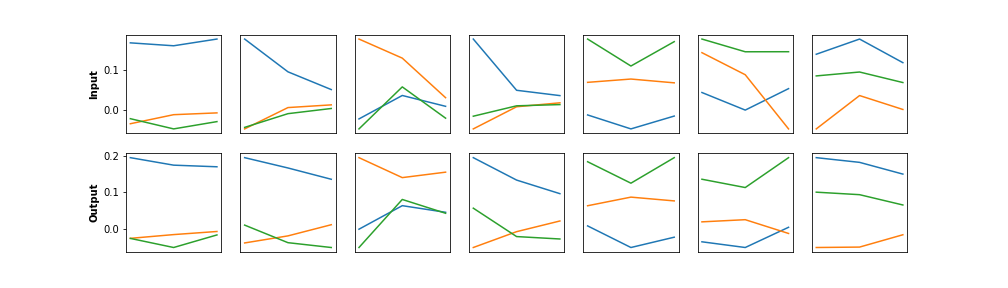
\includegraphics[width=\textwidth]{imagenes/Cap5/resultado_nn}
            \caption{Results of \textbf{NN\_33} network}
            \label{fig:res_nn}
        \end{subfigure}       
        \begin{subfigure}[h]{0.99\textwidth} 
            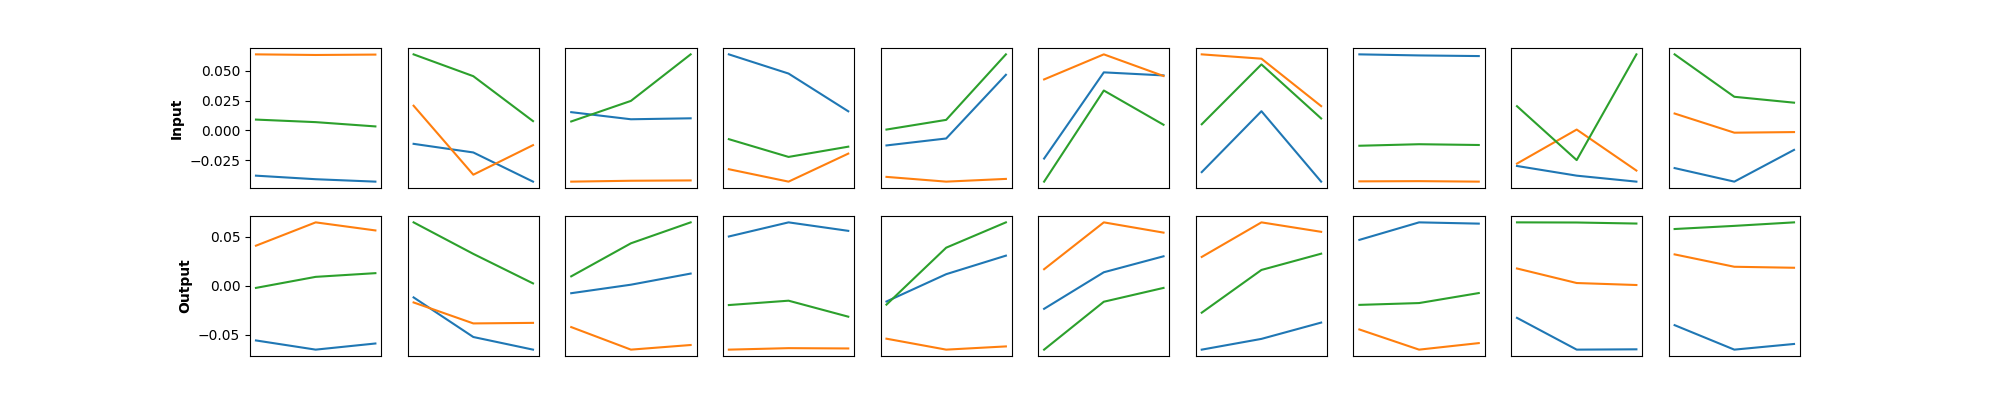
\includegraphics[width=\textwidth]{imagenes/Cap5/resultado_cnn}
            \caption{Results of \textbf{CNN\_33} network}
            \label{fig:res_cnn}
        \end{subfigure}
        
        \begin{subfigure}[h]{0.99\textwidth} 
            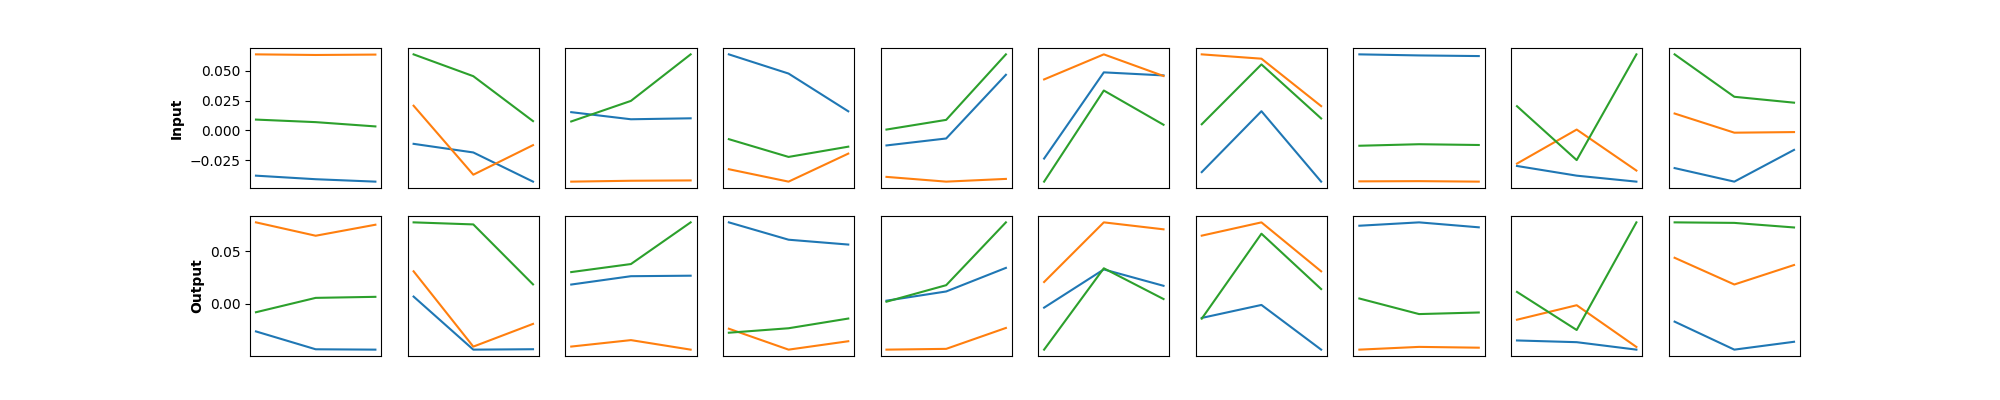
\includegraphics[width=\textwidth]{imagenes/Cap5/resultado_rnn}
            \caption{Results of \textbf{RNN\_33} network}
            \label{fig:res_rnn}
        \end{subfigure}     
        \end{varwidth}}
        \caption{Results (Own elaboration).}
        
		\label{fig:res_autoencoders}
    \end{figure}


\vspace{5mm} %5mm vertical space

Once the normal behavior model has been defined, the method of detecting outliers can be chosen.
%Una vez definido como est\'{a} constituido el modelo del comportamiento normal se puede proceder con la elecci\'{o}n del m\'{e}todo de detecci\'{o}n de valores at\'{i}picos.

\subsection{Anomaly detection method}

At the beginning of this section, three different approaches to anomaly detection were defined: thresholding, applying isolation forests, and finally applying One-Class SVM.
%Al inicio de esta secci\'{o}n se defini\'{o} tres diferentes enfoques para la detecci\'{o}n de anomal\'{i}as: la umbralizaci\'{o}n, la aplicaci\'{o}n de bosques de aislamiento y finalmente la aplicaci\'{o}n de SVM para una clase.

\subsubsection{Thresholding}

This technique is based on the definition of a threshold to determine if reconstruction error obtained by autoencoder (normal behavior model) is high enough to be considered an outlier. Therefore reconstruction error equation must first be defined for model. In the present work, reconstruction error is defined according to equation \ref{eqn:error_rec}, where $x_{i}$ represents the real value (autoencoder's input) and $\hat{x_{i}}$ represents the value obtained by autoencoder (autoencoder's output).
%Esta t\'{e}cnica se basa en la definici\'{o}n de un umbral para determinar si el error de reconstrucci\'{o}n  que obtiene el autoencoder (modelo del comportamiento normal) es lo suficientemente alto como para considerarse un valor at\'{i}pico. Por lo tanto primero se debe definir la ecuaci\'{o}n del error de reconstrucci\'{o}n para el modelo. En el presente trabajo el error de reconstrucci\'{o}n se define seg\'{u}n la ecuaci\'{o}n \ref{eqn:error_rec}, donde $x_{i}$ representa el valor real (entrada del autoencoder) y $\hat{x_{i}}$ representa el valor obtenido por el autoencoder (salida del autoencoder).

\begin{equation}
\textup{Reconstruction error} = S_{z} = |x_{i} - \hat{x_{i}}|^{2} 
\label{eqn:error_rec}
\end{equation}

Figure \ref{fig:codos} shows the curve of reconstruction errors obtained with normal behavior model for normal samples set.
%En la Figura \ref{fig:codos} se muestra la curva de los errores de reconstrucci\'{o}n obtenidos con el modelo del compotamiento normal para el conjunto de muestras normales.

\begin{figure}[H]
        \centering
            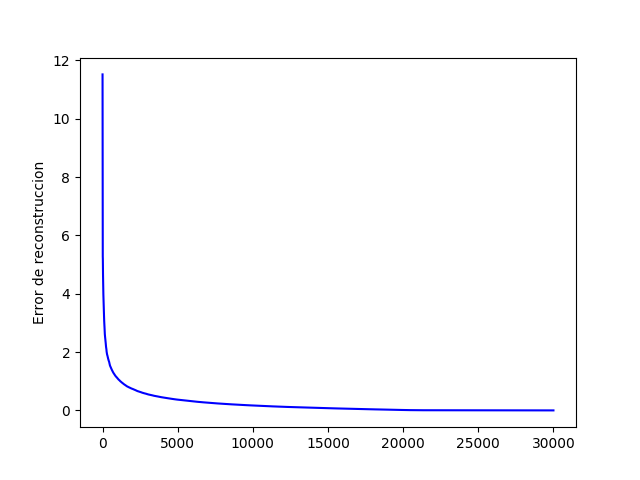
\includegraphics[width=0.75\textwidth, frame]{imagenes/Cap5/codos}
        \caption{Curve of reconstruction values obtained with the normal behavior model (Own elaboration).}
		\label{fig:codos}
    \end{figure}

Once the reconstruction equation has been defined, a threshold must be defined capable of detecting as many anomalies as possible. This task can be made simple in a supervised learning environment, however automating this task in an unsupervised learning context is a challenge that can be difficult to overcome. In present work a technique based on finding an \textit{elbow point} of a curve was used, which in this case the curve is built based on autoencoder reconstruction errors.
%Una vez definido la ecuaci\'{o}n de reconstrucci\'{o}n, se debe definir un umbral capaz de poder detectar la mayor cantidad de anomal\'{i}as posibles. Esta tarea puede tornarse simple en un entorno de aprendizaje supervisado, sin embargo automatizar esta tarea en un contexto de aprendizaje no supervisado es un desaf\'{i}o que puede ser dif\'{i}cil de sobrellevar. En el presente trabajo se us\'{o} una t\'{e}cnica basada en encontrar un \textit{Punto de codo} de una curva, que en este caso la curva est\'{a} construida en base a los errores de reconstrucci\'{o}n del autoencoder.

\vspace{5mm} %5mm vertical space

There are different ways to find the elbow point, however in this work a Python tool was used, which automates this task, called Kneedle. This tool returns the inflection point of curve function obtained by values' set provided $x$ and $y$, it should be noted that elbow point is maximum curvature's point, on the other hand this tool has a sensitivity parameter (S), this parameter allows adjusting how aggressive you want to be when detecting elbows, the smallest values for S detect elbows faster, while the largest are more conservative, that is, S is a measure of how many ''flat'' points are expect to see unmodified data curve before declaring an elbow.
% https://github.com/arvkevi/kneed
%Existen diferentes formas de hallar el punto de codo, sin embargo en este trabajo se utiliz\'{o} una herramienta de Python, que automatiza esta tarea, llamada Kneedle. Esta herramienta devuelve el punto de inflexi\'{o}n de la funci\'{o}n de la curva obtenida por el conjunto de valores proporcionado \textit{x} y \textit{y}, cabe recalcar que el punto de codo es el punto de m\'{a}xima curvatura, por otra parte esta herramienta cuenta con un par\'{a}metro de sensibilidad (S), este par\'{a}metro permite ajustar qu\'{e} tan agresivo se desea ser al detectar codos, los valores m\'{a}s peque\~{n}os para S detectan los codos m\'{a}s r\'{a}pido, mientras que los m\'{a}s grandes son m\'{a}s conservadores, es decir, S es una medida de cu\'{a}ntos puntos ''planos'' se espera ver en la curva de datos sin modificar antes de declarar un codo.

\vspace{5mm} %5mm vertical space

Thus, in present project, experiments were carried out with different sensitivity values to find the most appropriate elbow for data set with which we worked. Figure \ref{fig:zoom_codos} shows different elbows found for sensitivity values provided (values between 0 and 2).
%De esta manera en el presente proyecto se realiz\'{o} experimentos con diferentes valores de sensibilidad para encontrar el codo m\'{a}s adecuado para el conjunto de datos con el que se trabajo. En la Figura \ref{fig:zoom_codos}, se muestra los diferentes codos hallados para los valores de sensibilidad proporcionados (valores entre 0 y 2).

\begin{figure}[H]
        \centering
            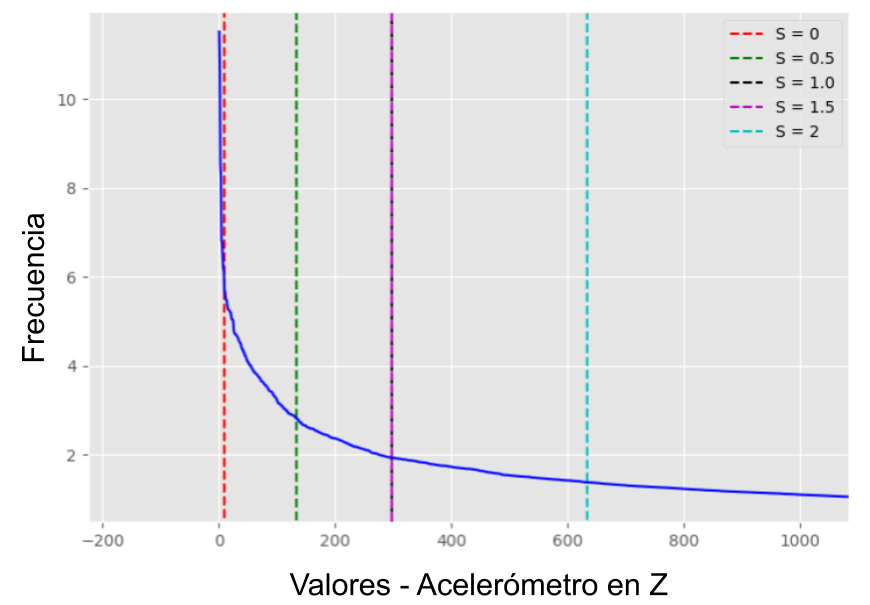
\includegraphics[width=0.75\textwidth, frame]{imagenes/Cap5/zoom_codos}
        \caption{Results of obtaining elbows with different Sensitivity values, for reconstruction values obtained with normal behavior model (Own elaboration).}
		\label{fig:zoom_codos}
\end{figure}

Once the elbows were obtained, each of them was evaluated. Table \ref{table:evaluacion_codos} shows threshold, the confusion matrix values, the sensitivity and specificity for each elbow. Confusion matrix values are result of applying the threshold of each elbow to reconstruction errors obtained from total data set (normal and anomalous data set equivalent to 44204 data).
%Una vez obtenidos los codos se realiz\'{o} la evaluaci\'{o}n de cada uno de ellos, en el Cuadro \ref{table:evaluacion_codos} se presentan el umbral, los valores de la matriz de confusi\'{o}n, la sensibilidad y especifidad para cada codo. Los valores de la matriz de confusi\'{o}n son el resultado de aplicar el umbral de cada codo a los errores de reconstrucci\'{o}n obtenidos del conjunto de datos total (conjunto de datos normal y anormal equivalente a 44204 datos).

\begin{table}[H]
\centering
\begin{center}
\begin{tabular}{|l|r|r|r|r|r|r|r|}
\hline
\textbf{S} & \multicolumn{1}{l|}{\textbf{Threshold}} & \multicolumn{1}{l|}{\textbf{VP}} & \multicolumn{1}{l|}{\textbf{VN}}& \multicolumn{1}{l|}{\textbf{FN}}& \multicolumn{1}{l|}{\textbf{FP}} & \multicolumn{1}{l|}{\textbf{Sensitivity}} & \multicolumn{1}{l|}{\textbf{Specificity}} \\ \hline
0.0 & 5.665 & \cellcolor[HTML]{AADD99} 92 & \cellcolor[HTML]{AADD99} 43993 & \cellcolor[HTML]{FFCE93} 72 & \cellcolor[HTML]{FFCE93} 47 & 0.5610 & 0.9989 \\ \hline
0.5  & 2.806 & \cellcolor[HTML]{AADD99} 111 & \cellcolor[HTML]{AADD99} 43814 & \cellcolor[HTML]{FFCE93} 53 & \cellcolor[HTML]{FFCE93} 226 & 0.6768 & 0.9949 \\ \hline
1.0 &  1.920 & \cellcolor[HTML]{AADD99} 120 & \cellcolor[HTML]{AADD99} 43562 & \cellcolor[HTML]{FFCE93} 44 & \cellcolor[HTML]{FFCE93} 478 & 0.7317 & 0.9891 \\ \hline
2.0 & 1.369	 & \cellcolor[HTML]{AADD99} 128 & \cellcolor[HTML]{AADD99} 43100  & \cellcolor[HTML]{FFCE93} 36 & \cellcolor[HTML]{FFCE93} 940 & 0.7805 & 0.9787 \\ \hline
\end{tabular}
\end{center}
\caption{Assessment of anomalies' detection for each elbow obtained with the different sensitivity values (Own elaboration).}
\label{table:evaluacion_codos}
\end{table}

According to results shown in Table \ref{table:evaluacion_codos}, it can be said that when the threshold is smaller the sensitivity (proportion of anomalies correctly detected as anomalies) increases, however, in turn it reduces the specificity (proportion of normal values correctly detected as normal values). Therefore, an intermediate point must be found, where as many anomalies as possible can be detected and the number of false positives (normal data that are detected as anomalies) reduced as much as possible. Thus, the most appropriate threshold for proposed objective was 2.806, since 111 abnormalities out of 164 are detected with this threshold and false positives are approximately twice the outliers detected.
%Seg\'{u}n los resultados que se muestran en el Cuadro \ref{table:evaluacion_codos} se puede decir que mientras m\'{a}s peque\~{n}o es el umbral la sensibilidad (proporci\'{o}n de anomal\'{i}as detectadas correctamente como anomal\'{i}as) incrementa, sin embargo, a su vez reduce la especifidad (proporci\'{o}n de valores normales correctamente detectados como valores normales). Por lo tanto se debe hallar un punto intermedio, donde se pueda detectar la mayor cantidad de anomal\'{i}as posibles y reducir en lo posible la cantidad de falsos positivos (datos normales que son detectados como anomal\'{i}as). De esta forma el umbral m\'{a}s adecuado para el objetivo planteado fue 2.806, ya que con este umbral se detecta 111 anomal\'{i}as de 164 y los falsos positivos son aproximadamente el doble de los valores at\'{i}picos detectados. 

\vspace{5mm} %5mm vertical space

It follows that, to automatically detect threshold, the use of 0.5 as parameter $S$ is the most appropriate, however if you want to increase  percentage of anomalies detection at the cost of increasing the number of false positives, you can use a higher value 0.5 for $S$ and if you want the fewest possible false positives, a value less than 0.5 should be used.
%De ello se deduce que, para detectar autom\'{a}ticamente el umbral el uso de 0.5 como par\'{a}metro S es el m\'{a}s adecuado, sin embargo si se desea incrementar el porcentaje de detecci\'{o}n de anomal\'{i}as a costa de incrementar el n\'{u}mero de falsos positivos se puede usar un valor mayor a 0.5 para S y en caso de querer la menor cantidad de falsos positivos posibles se debe usar un valor menor a 0.5.

\subsubsection{Isolation Forest}

Before presenting how experiments with this algorithm will be carried out, it is necessary to illustrate its operation in more detail. Therefore Figure \ref{fig:isolartion-forest} depicts how an anomalous data point is expected to quickly become isolated with the use of this algorithm, whereas a normal data point needs more partitions to be isolated.
%Antes de presentar como se llevar\'{a} a cabo los experimentos con este algoritmo, es necesario ilustrar m\'{a}s detalladamente el funcionamiento del mismo. Por lo tanto la Figura \ref{fig:isolartion-forest} representa c\'{o}mo se espera que un punto de datos anómalo se aísle rápidamente con el uso de este algoritmo, mientras que un punto de datos normal necesita más particiones para poder ser aislado.

\begin{figure}[h!]
  \begin{center}	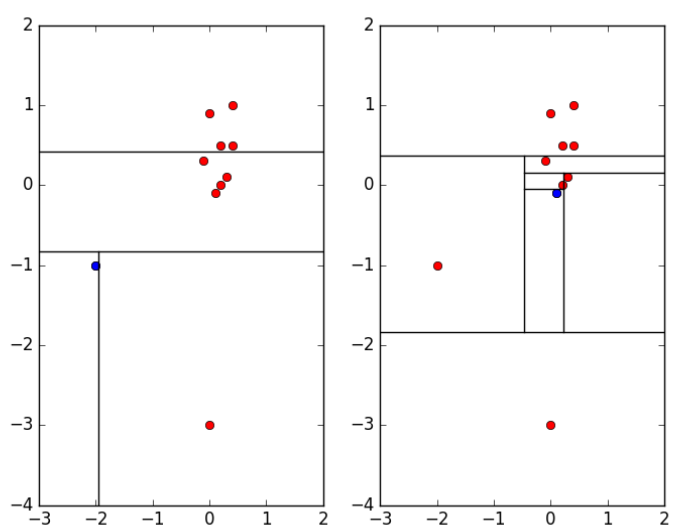
\includegraphics[width=0.75\textwidth, frame]{imagenes/Cap5/isolation-forest}
  \caption{The figure on left shows the isolation of an anomaly, requiring only three partitions. On right, isolation of a normal point requires six partitions \protect\cite{Reference60}.} 
  \label{fig:isolartion-forest}
  \end{center}
\end{figure}

Once isolation forest's operation has been briefly detail, the different approaches to experiments to be carried out with Isolation Forest can be continued.
%Una vez detallado resumidamente el funcionamiento de los bosques de aislamiento se puede proseguir con los diferentes enfoques de los experimentos que se realizar\'{a} con Isolation Forest.

\vspace{5mm} %5mm vertical space

There are two approaches that can be done with this technique; first one trains the model with compressed values of autoencoder's encoder and second one trains with autoencoder reconstruction errors. The following is a graph (See Figure \ref{fig:autoencoder}) of autoencoder (normal behavior model) in order to have a better understanding of how experiments will be carried out both for isolation forests and for One-Class SVM.
%Existen dos enfoques que pueden realizarse con esta t\'{e}cnica; el primero entrena el modelo con los valores compresos del codificador del autoencoder y el segundo se entrena con los errores de reconstrucci\'{o}n del autoencoder. A continuaci\'{o}n se presenta una gr\'{a}fica (Ver Figura \ref{fig:autoencoder}) del autoencoder (modelo del comportamiento normal) con el fin de tener un mejor entendimiento de c\'{o}mo se realizar\'{a}n los experimentos tanto para los bosques de aislamiento como para los SVM de una clase.

\begin{figure}[H]
        \centering
            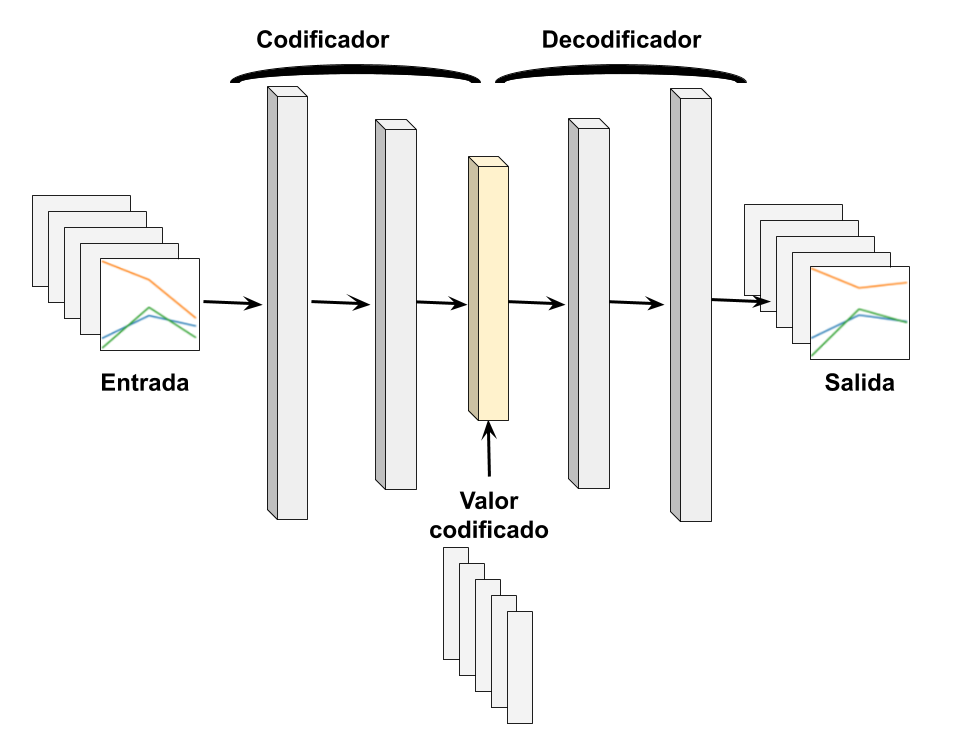
\includegraphics[width=0.75\textwidth, frame]{imagenes/Cap5/autoencoder}
        \caption{Graphical representation of normal behavior model or autoencoder (Own elaboration).}
		\label{fig:autoencoder}
\end{figure}

\begin{itemize}
\item \textbf{\textit{Isolation forest for encoded values: }}This technique trains an isolation forest model with the encoded values (using autoencoder's encoder, see Figure \ref{fig:autoencoder}) of normal training set. For experimentsm IsolationForest class of \textsc{scikit-learn} was used, this class has a parameter called \textsc{contamination} which serves to define how much of data set is contaminated, that is, it defines how much of training data can be outliers; in present investigation, several tests were carried out with different values for contamination parameter. Table  \ref{table:evaluacion_IF_encoded} presents the results, where it is evident that none of results is encouraging, since the number of anomalies detected is very low for the three cases with which it was experimented.
%\item \textbf{\textit{Isolation forest para valores codificados: }}Esta t\'{e}cnica entrena un modelo de bosque de aislamiento con los valores codificados (mediante el codificador del autoencoder, ver Figura \ref{fig:autoencoder}) del conjunto de entrenamiento normal. Para los experimentos se utiliz\'{o} la clase IsolationForest de \textsc{scikit-learn}, esta clase tiene un par\'{a}metro llamado \textsc{contaminaci\'{o}n} el cual sirve para definir que cantidad del conjunto de datos esta contaminado, es decir, define que cantidad de los datos de entrenamiento pueden ser valores at\'{i}picos; en la presente investigaci\'{o}n se realiz\'{o} varias pruebas con diferentes valores para el par\'{a}metro contaminaci\'{o}n. En el Cuadro \ref{table:evaluacion_IF_encoded} se presenta los resultados, donde se evidencia que ninguno de los resultados es alentador, ya que la cantidad de anomal\'{i}as detectadas es muy baja para los tres casos con los que se experimento.

\begin{table}[H]
\centering
\begin{center}
\begin{tabular}{|l|r|r|r|r|r|r|r|}
\hline
\textbf{Contamination (C)} & \multicolumn{1}{l|}{\textbf{VP}} & \multicolumn{1}{l|}{\textbf{VN}}& \multicolumn{1}{l|}{\textbf{FN}}& \multicolumn{1}{l|}{\textbf{FP}} & \multicolumn{1}{l|}{\textbf{Sensitivity}} & \multicolumn{1}{l|}{\textbf{Specificity}} \\ \hline
0.0025 & \cellcolor[HTML]{AADD99} 3 & \cellcolor[HTML]{AADD99} 43944 & \cellcolor[HTML]{FFCE93} 161 & \cellcolor[HTML]{FFCE93} 96 & 0.0183 & 0.9978 \\ \hline
0.0050 & \cellcolor[HTML]{AADD99} 17 & \cellcolor[HTML]{AADD99} 43817 & \cellcolor[HTML]{FFCE93} 147 & \cellcolor[HTML]{FFCE93} 223 & 0.1037 & 0.9949 \\ \hline
0.0075 & \cellcolor[HTML]{AADD99} 17 & \cellcolor[HTML]{AADD99} 43738 & \cellcolor[HTML]{FFCE93} 147 & \cellcolor[HTML]{FFCE93} 302 & 0.1037 & 0.9931 \\ \hline
\end{tabular}
\end{center}
\caption{Evaluation of anomalies' detection using Isolation forest for compressed values (Own elaboration).}
\label{table:evaluacion_IF_encoded}
\end{table}

\item \textbf{\textit{Isolation forest for reconstruction errors: }}For this technique, isolation forest training was performed with the difference of the input values with the values obtained by autoencoder (See Figure \ref{fig:error}), it should be clarified that the difference mentioned above will also be called Error reconstruction in this and the next subsection. Results of this technique for different contamination values are presented in Table \ref{table:evaluacion_IF_errores_reconstruccion}, where these results can be considered as optimal, since they range between 62 and 67\% of correct anomaly detections, in addition to presenting a really high specificity of approximately 99\%, which means that these models have a low false positive rate.
%\item \textbf{\textit{Isolation forest para errores de reconstrucci\'{o}n: }}Para esta t\'{e}cnica se realiz\'{o} el entrenamiento del bosque de aislamiento con la diferencia de los valores de entrada con los valores obtenidos por el autoencoder (Ver Figura \ref{fig:error}), cabe aclarar que la diferencia mencionada anteriormente tambi\'{e}n ser\'{a} llamada \textit{Error de reconstrucci\'{o}n} tanto en esta como en la siguiente subsecci\'{o}n. Los resultados de esta t\'{e}cnica para diferentes valores de contaminaci\'{o}n se presentan en el Cuadro \ref{table:evaluacion_IF_errores_reconstruccion}, donde estos resultados se pueden considerar como \'{o}ptimos, debido a que oscilan entre 62 y 67\% de detecciones correctas de anomal\'{i}as, adem\'{a}s de presentar una especificidad realmente alta, del 99\% aproximadamente, lo cual quiere decir que estos modelos presentan una baja tasa de falsos positivos. 

\begin{figure}[H]
        \centering
            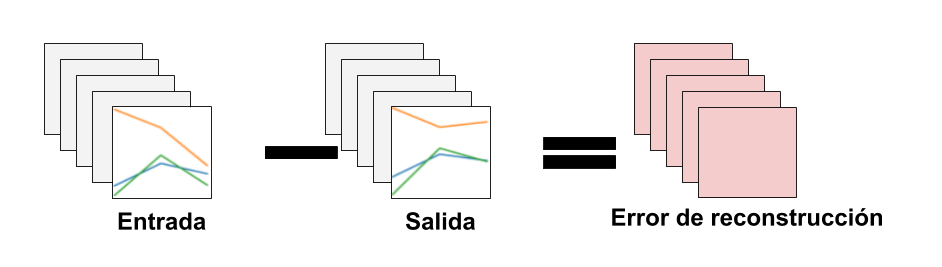
\includegraphics[width=0.75\textwidth, frame]{imagenes/Cap5/error}
        \caption{Graphical representation of reconstruction error used for the training of isolation forests and One-Class SVM (Own elaboration).}
		\label{fig:error}
\end{figure}

\begin{table}[H]
\centering
\begin{center}
\begin{tabular}{|l|r|r|r|r|r|r|r|}
\hline
\textbf{Contamination (C)} & \multicolumn{1}{l|}{\textbf{VP}} & \multicolumn{1}{l|}{\textbf{VN}}& \multicolumn{1}{l|}{\textbf{FN}}& \multicolumn{1}{l|}{\textbf{FP}} & \multicolumn{1}{l|}{\textbf{Sensitivity}} & \multicolumn{1}{l|}{\textbf{Specificity}} \\ \hline
0.0025 & \cellcolor[HTML]{AADD99} 103 & \cellcolor[HTML]{AADD99} 43898 & \cellcolor[HTML]{FFCE93} 61 & \cellcolor[HTML]{FFCE93} 142 & 0.6280 & 0.9968 \\ \hline
0.0050 & \cellcolor[HTML]{AADD99} 108 & \cellcolor[HTML]{AADD99} 43792 & \cellcolor[HTML]{FFCE93} 56 & \cellcolor[HTML]{FFCE93} 248 & 0.6585 & 0.9944 \\ \hline
0.0075 & \cellcolor[HTML]{AADD99} 111 & \cellcolor[HTML]{AADD99} 43688 & \cellcolor[HTML]{FFCE93} 53 & \cellcolor[HTML]{FFCE93} 352 & 0.6768 & 0.9920 \\ \hline
\end{tabular}
\end{center}
\caption{Evaluation of anomaly detection using Isolation forest for reconstruction errors (Own elaboration).}
\label{table:evaluacion_IF_errores_reconstruccion}
\end{table}
\end{itemize}

\subsubsection{One-Class SVM}

In the same way as in isolation forests, two different types of experiments were performed with One-Class SVM, each of which is detailed below.
%De la misma forma que en los bosques de aislamiento, se realiz\'{o} dos diferentes tipos de experimentos con One-Class SVM, a continuaci\'{o}n se detalla cada uno de ellos.

\begin{itemize}
\item \textbf{\textit{One-Class SVM for encoded values: }}A one-class SVM model be trained for compressed values obtained by autoencoder; experiments were performed using OneClassSVM class of \textsc{scikit-learn}, where there are different parameters that can be customized, for present investigation different kernels were tested, thus obtaining the results shown in Table \ref{table:evaluacion_SVM_encoded}, where clearly none of obtained results could be taken into account to be the method of detection conduction anomalies since the sensitivity in none of cases is greater than 50\%.
%\item \textbf{\textit{One-Class SVM para valores codificados: }}Se debe entrenar un modelo SVM de una clase para los valores compresos obtenidos por el autoencoder; los experimentos fueron realizados usando la clase OneClassSVM de \textsc{scikit-learn}, donde se tiene diferentes par\'{a}metros que pueden ser personalizados, para la presente investigaci\'{o}n se prob\'{o} diferentes kernels, obteniendo as\'{i} los resultados que se muestran en el Cuadro \ref{table:evaluacion_SVM_encoded}, donde claramente ninguno de los resultados obtenidos podr\'{i}a ser tomado en cuenta para ser el m\'{e}todo de detecci\'{o}n de anomal\'{i}as de conducci\'{o}n ya que la sensibilidad en ninguno de los casos es superior a 50\%.

\begin{table}[H]
\centering
\begin{center}
\begin{tabular}{|l|r|r|r|r|r|r|r|}
\hline
\textbf{Kernel} & \multicolumn{1}{l|}{\textbf{VP}} & \multicolumn{1}{l|}{\textbf{VN}}& \multicolumn{1}{l|}{\textbf{FN}}& \multicolumn{1}{l|}{\textbf{FP}} & \multicolumn{1}{l|}{\textbf{Sensitivity}} & \multicolumn{1}{l|}{\textbf{Specificity}} \\ \hline
rbf & \cellcolor[HTML]{AADD99} 49 & \cellcolor[HTML]{AADD99} 41746 & \cellcolor[HTML]{FFCE93} 115 & \cellcolor[HTML]{FFCE93} 2294 & 0.2988 & 0.9479 \\ \hline
poly & \cellcolor[HTML]{AADD99} 56 & \cellcolor[HTML]{AADD99} 22532 & \cellcolor[HTML]{FFCE93} 108 & \cellcolor[HTML]{FFCE93} 21508 & 0.3415 & 0.5116 \\ \hline
sigmoid & \cellcolor[HTML]{AADD99} 13 & \cellcolor[HTML]{AADD99} 42378 & \cellcolor[HTML]{FFCE93} 151 & \cellcolor[HTML]{FFCE93} 1662 & 0.0793 & 0.9623 \\ \hline
\end{tabular}
\end{center}
\caption{Anomaly detection evaluation using One-Class SVM for compressed values (Own elaboration).}
\label{table:evaluacion_SVM_encoded}
\end{table}

\item \textbf{\textit{One-Class SVM for reconstruction errors: }}Like one of experiments that were performed with Isolation Forest, in this technique the reconstruction errors are used (See Figure \ref{fig:error}) to carry out training of the One-Class SVM model. As in experiments carried out in previous technique, different tests were carried out with different types of kernel, the follow Table \ref{table:evaluacion_SVM_error} presents results obtained by experiments.
%\item \textbf{\textit{One-Class SVM para los errores de reconstrucci\'{o}n: }}Al igual que uno de los experimentos que se realiz\'{o} con Isolation Forest, en esta t\'{e}cnica se usa los errores de reconstrucci\'{o}n (Ver Figura \ref{fig:error}) para realizar el entrenamiento del modelo SVM de una clase. Como en los experimentos realizados en la anterior t\'{e}cnica se realiz\'{o} diferentes pruebas con distintos tipos de kernel, a continuaci\'{o}n en el Cuadro \ref{table:evaluacion_SVM_error} se presenta los resultados obtenidos en los experimentos.

\begin{table}[H]
\centering
\begin{center}
\begin{tabular}{|l|r|r|r|r|r|r|r|}
\hline
\textbf{Kernel} & \multicolumn{1}{l|}{\textbf{VP}} & \multicolumn{1}{l|}{\textbf{VN}}& \multicolumn{1}{l|}{\textbf{FN}}& \multicolumn{1}{l|}{\textbf{FP}} & \multicolumn{1}{l|}{\textbf{Sensitivity}} & \multicolumn{1}{l|}{\textbf{Specificity}} \\ \hline
rbf & \cellcolor[HTML]{AADD99} 134 & \cellcolor[HTML]{AADD99} 41887 & \cellcolor[HTML]{FFCE93} 30 & \cellcolor[HTML]{FFCE93} 2153 & 0.8170 & 0.9511 \\ \hline
poly & \cellcolor[HTML]{AADD99} 97 & \cellcolor[HTML]{AADD99} 1559 & \cellcolor[HTML]{FFCE93} 67 & \cellcolor[HTML]{FFCE93} 42481 & 0.5915 & 0.0354 \\ \hline
sigmoid & \cellcolor[HTML]{AADD99} 123 & \cellcolor[HTML]{AADD99} 1683 & \cellcolor[HTML]{FFCE93} 41 & \cellcolor[HTML]{FFCE93} 42357 & 0.7500 & 0.0382 \\ \hline
\end{tabular}
\end{center}
\caption{Anomaly detection evaluation using One-Class SVM for autoencoder's reconstruction error (Own elaboration).}

\label{table:evaluacion_SVM_error}
\end{table}

Observing results of Table \ref{table:evaluacion_SVM_error}, it can be seen that the sensitivity, or number of anomalies detected correctly, was significantly increased, however, it drastically reduced the specificity since in some cases it only reaches 3.5\%, which is very far from objective pursued in the present work.
%Observando los resultados del Cuadro \ref{table:evaluacion_SVM_error} se puede notar que se aument\'{o} notablemente la sensibilidad, o cantidad de anomal\'{i}as detectadas correctamente, sin embargo, redujo dr\'{a}sticamente la especificidad ya que en algunos casos tan solo llega a un 3.5\%, lo cual es muy alejado al objetivo que se persigue en el presente trabajo.

\end{itemize}

\subsubsection{Evaluation of the anomaly detection method}

Once the different types of experiments had been carried out, the best exponent of each type was evaluated, in order to choose the most suitable one for this investigation. Below is a Table \ref{table:evaluacion_metodo_anomalias} with results of the best representatives for each type of technique.
%Una vez realizado los diferentes tipos de experimentos, se evalu\'{o} el mejor exponente de cada tipo, con el fin de elegir el m\'{a}s adecuado para la investigaci\'{o}n. A continuaci\'{o}n se presenta un Cuadro \ref{table:evaluacion_metodo_anomalias} con los resultados de los mejores representantes por cada tipo de t\'{e}cnica.

\begin{table}[H]
\centering
\begin{center}
\begin{tabular}{|p{40mm}|r|r|r|r|r|r|r|}
\hline
\textbf{Method name} & \multicolumn{1}{l|}{\textbf{VP}} & \multicolumn{1}{l|}{\textbf{VN}}& \multicolumn{1}{l|}{\textbf{FN}}& \multicolumn{1}{l|}{\textbf{FP}} & \multicolumn{1}{l|}{\textbf{Sensitivity}} & \multicolumn{1}{l|}{\textbf{Specificity}} \\ \hline
Thresholding with S=0.5 & \cellcolor[HTML]{AADD99} 111 & \cellcolor[HTML]{AADD99} 43814 & \cellcolor[HTML]{FFCE93} 53 & \cellcolor[HTML]{FFCE93} 226 & 0.6768 & 0.9949 \\ \hline
Isolation Forest for reconstruction errors with C=0.0075 & \cellcolor[HTML]{AADD99} 111 & \cellcolor[HTML]{AADD99} 43688 & \cellcolor[HTML]{FFCE93} 53 & \cellcolor[HTML]{FFCE93} 352 & 0.6768 & 0.9920 \\ \hline
One-Class SVM for reconstruction errors with kernel RBF& \cellcolor[HTML]{AADD99} 134 & \cellcolor[HTML]{AADD99} 41887 & \cellcolor[HTML]{FFCE93} 30 & \cellcolor[HTML]{FFCE93} 2153 & 0.8170 & 0.9511 \\ \hline
\end{tabular}
\end{center}
\caption{Comparison of the best anomaly detection methods (own elaboration).}

\label{table:evaluacion_metodo_anomalias}
\end{table}

Obviously, the best anomaly detection result is the one obtained by SVM model for a class with a sensitivity of 81.7\%, however, this method has the disadvantage of having a high number of false positives, that is, for each anomaly detected, there will be approximately 13 false positive alerts, which is a very high value; and it is the main reason why this method is discarded.
%Evidentemente el mejor resultado de detecci\'{o}n de anomal\'{i}as es el que se obtuvo por el modelo SVM para una clase con una sensibilidad del 81.7\%, sin embargo, este m\'{e}todo presenta la desventaja de tener una alta cantidad de falsos positivos, es decir, por cada anomal\'{i}a detectada se tendr\'{a} aproximadamente 13 alertas por falsos positivos, lo cual es una valor muy alto; y es la principal raz\'{o}n por la que se descarta este m\'{e}todo.

\vspace{5mm} %5mm vertical space

Due to this, there are only two methods to compare, where both results are very similar; since these have a sensitivity of 67.68\%, on the other hand, the specificity has a small variation between both techniques, giving a slightly better result for the thresholding technique with 99.49\% compared to 99.20\%.
%Debido a esto s\'{o}lo quedan dos m\'{e}todos a comparar, donde ambos resultados son muy similares; ya que estos cuentan con una sensibilidad de 67.68\%, por otra parte la especificidad tiene una peque\~{n}a variaci\'{o}n entre ambas t\'{e}cnicas dando un resultado levemente mejor para la t\'{e}cnica de umbralizaci\'{o}n con 99.49\% frente a un 99.20\%.

\vspace{5mm} %5mm vertical space

At this point you can choose either of these two methods due to the similarities that both present. For reasons of simplicity, the isolation forest method was chosen in this study since this method makes it easier to detect anomalies because one can specify the amount of contamination expected from dataset, this is much more advantageous than the search for elbows with thresholding method since it has the disadvantage that it is really complex to define the threshold when we use an unsupervised approach, as is case in this stage, in addition to the fact that definition of threshold depends a lot on how clean or contaminated data set is, making the correct treatment more complex when applying this method.
%En este punto se puede elegir cualquiera de estos dos m\'{e}todos debido a las similitudes que ambos presentan. Por razones de simplificidad en este estudio se elegi\'{o} el m\'{e}todo de bosque de aislamiento ya que este m\'{e}todo hace m\'{a}s sencilla la detecci\'{o}n de anomal\'{i}as debido a que uno puede especificar la cantidad de contaminaci\'{o}n que se espera del conjunto de datos, esto es mucho m\'{a}s ventajoso que la busqueda de codos con el m\'{e}todo de umbralizaci\'{o}n ya que presenta la desventaja de que es realmente complejo definir el umbral cuando se trata esta t\'{e}cnica en un enfoque no supervisado, como es el caso de esta etapa, adem\'{a}s que la definici\'{o}n del umbral depende mucho de cu\'{a}n limpio o contaminado se encuentra el conjunto de datos, haciendo m\'{a}s complejo el correcto tratamiento al aplicar este m\'{e}todo.

\vspace{5mm} %5mm vertical space

Once the best methods for conforming the outlier detection mechanism have been chosen, this mechanism is formalized by means of a graph (See Figure \ref{fig:mecanismo}), which provides a visual representation of the flow of proposed anomaly detector; since it is important to know how it is composed and how it works, especially before carrying out its respective evaluation.
%Una vez elegido los mejores m\'{e}todos para conformar el mecanismo de detecci\'{o}n de valores at\'{i}picos, se procede a formalizar este mecanismo por medio de una gr\'{a}fica (Ver Figura \ref{fig:mecanismo}), la cual proporciona una representaci\'{o}n visual del flujo del detector de anomal\'{i}as propuesto; ya que es importante conocer como se compone y como funciona, especialmente antes de realizar su respectiva evaluaci\'{o}n. 

\begin{figure}[H]
        \centering
            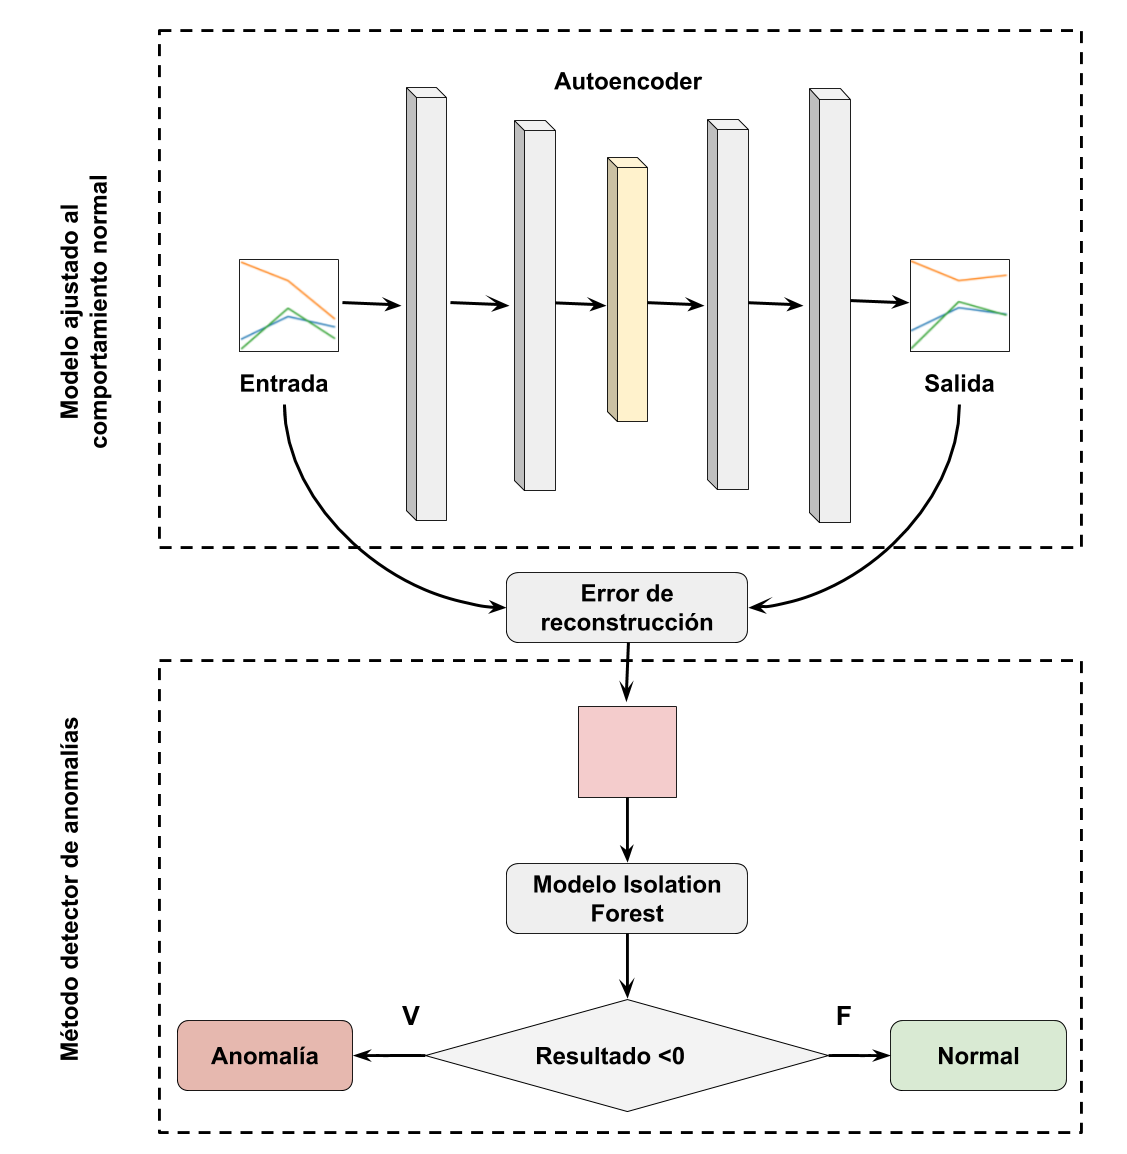
\includegraphics[width=0.92\textwidth, frame]{imagenes/Cap5/mecanismo}
        \caption{Anomaly detection mechanism (Own elaboration).}
		\label{fig:mecanismo}
\end{figure}

Looking at Figure \ref{fig:mecanismo}, the components that compose the anomaly detection mechanism can be clearly seen: the \textbf{normal behavior model} and the \textbf{anomaly detection method}. This mechanism works in a very simple way, firstly the autoencoder is provided with an input sequence with 3 steps for 3 principal components (it should be noted that input data has been previously pre-processed), this autoencoder returns reconstruction as output of the input, with which the reconstruction error is obtained (difference between real input and reconstructed value), this value is in turn the input of the isolation forest model, which can return two types of values ​​(-1 , 1); when this model returns the value 1, it means that input provided corresponds to a value considered normal, and if it returns -1, it means that this input is an anomaly, thus ending the flow of detection mechanism proposed in this work.
%Observando la Figura \ref{fig:mecanismo}, se puede notar claramente los componentes que conforman el mecanismo de detecci\'{o}n de anomal\'{i}as: el \textbf{modelo del comportamiento normal} y el \textbf{m\'{e}todo detector de anomal\'{i}as}. Este mecanismo funciona de una forma muy sencilla, en primer lugar se proporciona al autoencoder una secuencia de entrada con 3 pasos para 3 componentes principales (cabe aclarar que los datos de entrada han sido previamente pre-procesados), este autoencoder devuelve como salida la reconstrucci\'{o}n de la entrada, con la cual se obtiene el error de reconstrucci\'{o}n (diferencia entre la entrada real y el valor reconstruido), dicho valor es a su vez la entrada del modelo de bosque de aislamiento, el cual puede retornar dos tipos de valores (-1, 1); cuando este modelo retorna el valor 1 quiere decir que la entrada proporcionada corresponde a un valor considerado como normal y en caso de retornar -1 significa que dicha entrada es una anomal\'{i}a, terminando as\'{i} el flujo del mecanismo de detecci\'{o}n propuesto en el presente trabajo.

%\section{Resumen del cap\'{i}tulo}

%En este cap\'{i}tulo se ha detallado como est\'{a} conformado el conjunto de valores at\'{i}picos, que herramientas fueron utilizadas para el desarrollo de los experimentos. Por otra parte tambi\'{e}n se describi\'{o} detalladamente todos los tipos de experimentos realizados durante la investigaci\'{o}n y finalmente la elecci\'{o}n de los m\'{e}todos m\'{a}s adecuados para formar parte del mecanismo de detecci\'{o}n de anomal\'{i}as. En el siguiente cap\'{i}tulo se abordar\'{a} un an\'{a}lisis detallado de los resultados obtenidos por el mecanismo de detecci\'{o}n.
 